\documentclass[10pt]{iopart}

\usepackage{graphicx}
\graphicspath{{./figures/}}
%\usepackage[acronym]{glossaries}
\usepackage{acro}

\DeclareAcronym{cejst}{short=CEJST,
                       long=Climate and Energy Justice Screening Tool
}

\DeclareAcronym{ipcc}{short=IPCC,
                      long=International Panel on Climate Change
}

\DeclareAcronym{nsrdb}{short=NSRDB,
                       long=National Solar Radiation Database
}

\DeclareAcronym{nrel}{short=NREL,
                       long=National Renewable Energy Laboratory
}

\DeclareAcronym{lmi}{short=LMI,
                     long=low and moderate income
}

\DeclareAcronym{uhi}{short=UHI,
                     long=Urban Heat Island
}

\DeclareAcronym{ceja}{short=CEJA,
                      long=Climate and Equitable Jobs Act
}



\begin{document}

\title[Minimizing heatwave risk through an equitable distribution of solar panels]{Minimizing 
heatwave risk through an equitable distribution of solar panels}
 
 \author{
 Samuel G. Dotson $^1$$^*$, 
 Shannon R. Anderson $^2$, 
 Alankrita Sahay $^3$,
 Pranjali Borse  $^3$,
 Charumeghana Samantula  $^3$
 }
 
 \address{ $^1$ Department of Nuclear, Plasma, and Radiological Engineering, 
 University of Illinois Urbana-Champaign, Urbana IL, United States}
  \address{ $^2$ Department of  Natural Resources and Environmental Sciences, 
 University of Illinois Urbana-Champaign, Urbana IL, United States}
  \address{ $^3$ Department of Civil and Environmental Engineering, 
 University of Illinois Urbana-Champaign, Urbana IL, United States}
 \address{$^*$ Author to whom correspondence should be addressed}
 
 \ead{sgd2@illinois.edu}
 
 \begin{indented}
 \vspace{10pt}
 \item[]May 2022
 \end{indented}

 \begin{abstract}
 Testing abstract. \ac{cejst}. \ac{cejst}
 \end{abstract}
 
 \vspace{2pc}
\noindent{\it Keywords}: solar, heatwave, equity, energy justice, policy

\ioptwocol

\section{Introduction}

\section{Methods and Data}

\section{Results}
\begin{figure}[ht]
    \centering
    \label{fig:equity_map}
    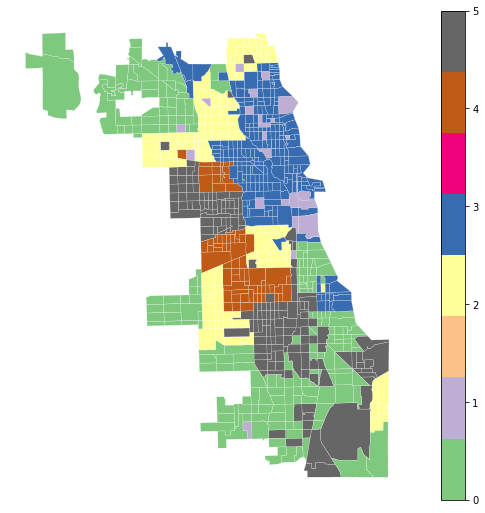
\includegraphics[width=\columnwidth]{cluster_map}
\end{figure}

\section{Discussion}

\section{Conclusion}
 
 \end{document}